%-------------------------------------------------------------------------------
\chapter{Numerical experiment}
In this section we will show the results of the Burgers equation with a Dirichlet boundary conditions at the left side of the domain.

The considered Burgers equation reads:
\begin{align}
    \pdiff{u}{t} + \half \pdiff{u^2}{x} - \pdiff{}{x}\left( (\nu+\Psi) \pdiff{u}{x}\right)= 0, \qquad u>0. \label{eq:1d_advection_art_diff}
\end{align}
where
\begin{symbollist}
    \item[$u$] Convected velocity, $\bunit{\metre\per\second}$.
    \item[$\nu$] Constant diffusion coefficient, $\bunit{\square\metre\per\second}$.
    \item[$\Psi(t)$] Artificial diffusion coefficient, $\bunit{\square\metre\per\second}$.
\end{symbollist}
The prescribed boundary condition for the velocity reads
% reg_factor = 0.5 * (std::cos(M_PI * (treg - double(nst) * dt) / treg) + 1.0);
\begin{align}
    u(0,t) = u_{\it given}(t)
    \begin{cases}
        \half \left(\cos\left(\pi \frac{t_{reg} - t}{t_{reg}} \right) + 1\right) &\quad \text{if } t < t_{reg},
        \\
        1 &\quad \text{if } t \geq t_{reg},
    \end{cases}
    \label{eq:1d_burgers_boundary_condition}
\end{align}
where
\begin{symbollist}
    \item[$t_{reg}$] The regularization time for the given time-series, [\si{\second}]
    \nomenclature{$t_{reg}$}{\si{\second}}{The regularization time for the given time-series}
    \item[$u_{\it given}(t)$] Prescribed (given) time-series at the boundary.
\end{symbollist}

%-------------------------------------------------------------------------------
\section{Experiments without/with artifcial viscosity}
In this section results of simulations without and with artificial viscosity will be compared.
Several test cases where the viscosity is well resolved on the grid and several cases where is not.

%--------------------------------------------------------------------------------
\paragraph*{Numerical experiment}

The numerical experiment is performed with the following parameters:
\begin{itemize}
    \item Length of the domain, $L_x = \bqty{20000}{\metre}$
    \item Grid size, $\Dx = \bqty{10}{\metre}$
    \item Start time, $t_{start} = \bqty{0}{\second}$
    \item End time, $t_{stop} = \bqty{4}{\hour}$
    \item Timestep, $\Dt = \bqty{5}{\second}$
    \item Regularization time for time-series, $t_{\it reg} = \bqty{1800}{\second}$
    \item Prescribed initial velocity, $u_{\it initial}(x,t) = \bqty{1}{\metre\per\second}$
    \item Prescribed velocity on boundary at $x=0$ is given by \autoref{eq:1d_burgers_boundary_condition}, with $u_{\it given} = \bqty{2}{\metre\per\second}$.
    \item No boundary is prescribed at $x=\bqty{20000}{\metre}$.
\end{itemize}
The speed of the fully developed shock wave for the inviscid Burgers equation is $u_{\it shock} =\bqty{1.5}{\metre\per\second}$ \citep[eq.\ 8.1.67]{Debnath2008}

%----------------------------------------------------------
\section[Experiment with viscosity of 20 m2/s]{Experiment with viscosity of \bqty{20}{\metre\square\per\second}}
\begin{figure}[H]
    \begin{subfigure}{0.49\textwidth}
        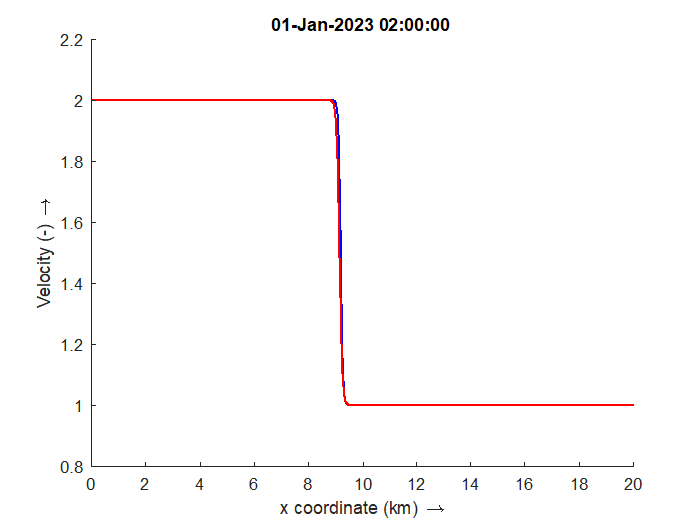
\includegraphics[width=\textwidth]{figures/nu020d0_velocity.png}
        \caption{Velocity along channel at $\bqty{2}{\hour}$.
        The blue line, without artificial viscosity and the red line with artificial velocity.
    }
    \end{subfigure}
    \hfill
    \begin{subfigure}{0.49\textwidth}
        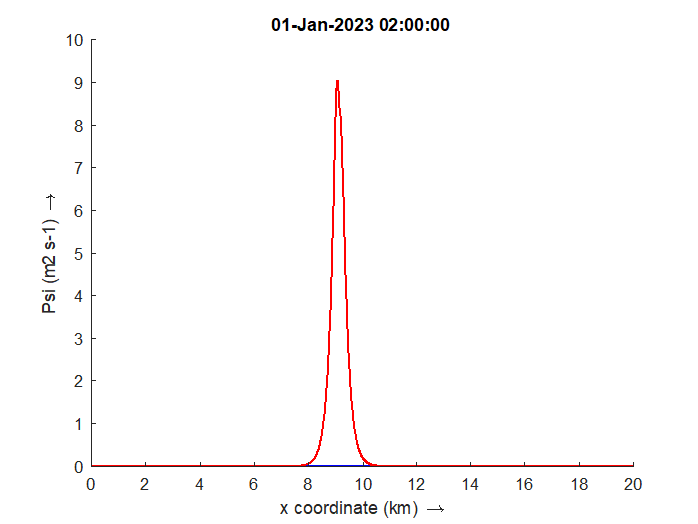
\includegraphics[width=\textwidth]{figures/nu020d0_psi.png}
        \caption{Used artificial viscoity $\Psi$ along channel at $\bqty{2}{\hour}$. The blue line, without artificial viscosity ($\equiv 0$) and the red line with artificial velocity.}
    \end{subfigure}
    \caption{Transect for velocity $\nu = \bqty{20}{\square\meter\per\second}$}
\end{figure}

\begin{figure}[H]
    \begin{subfigure}{0.49\textwidth}
        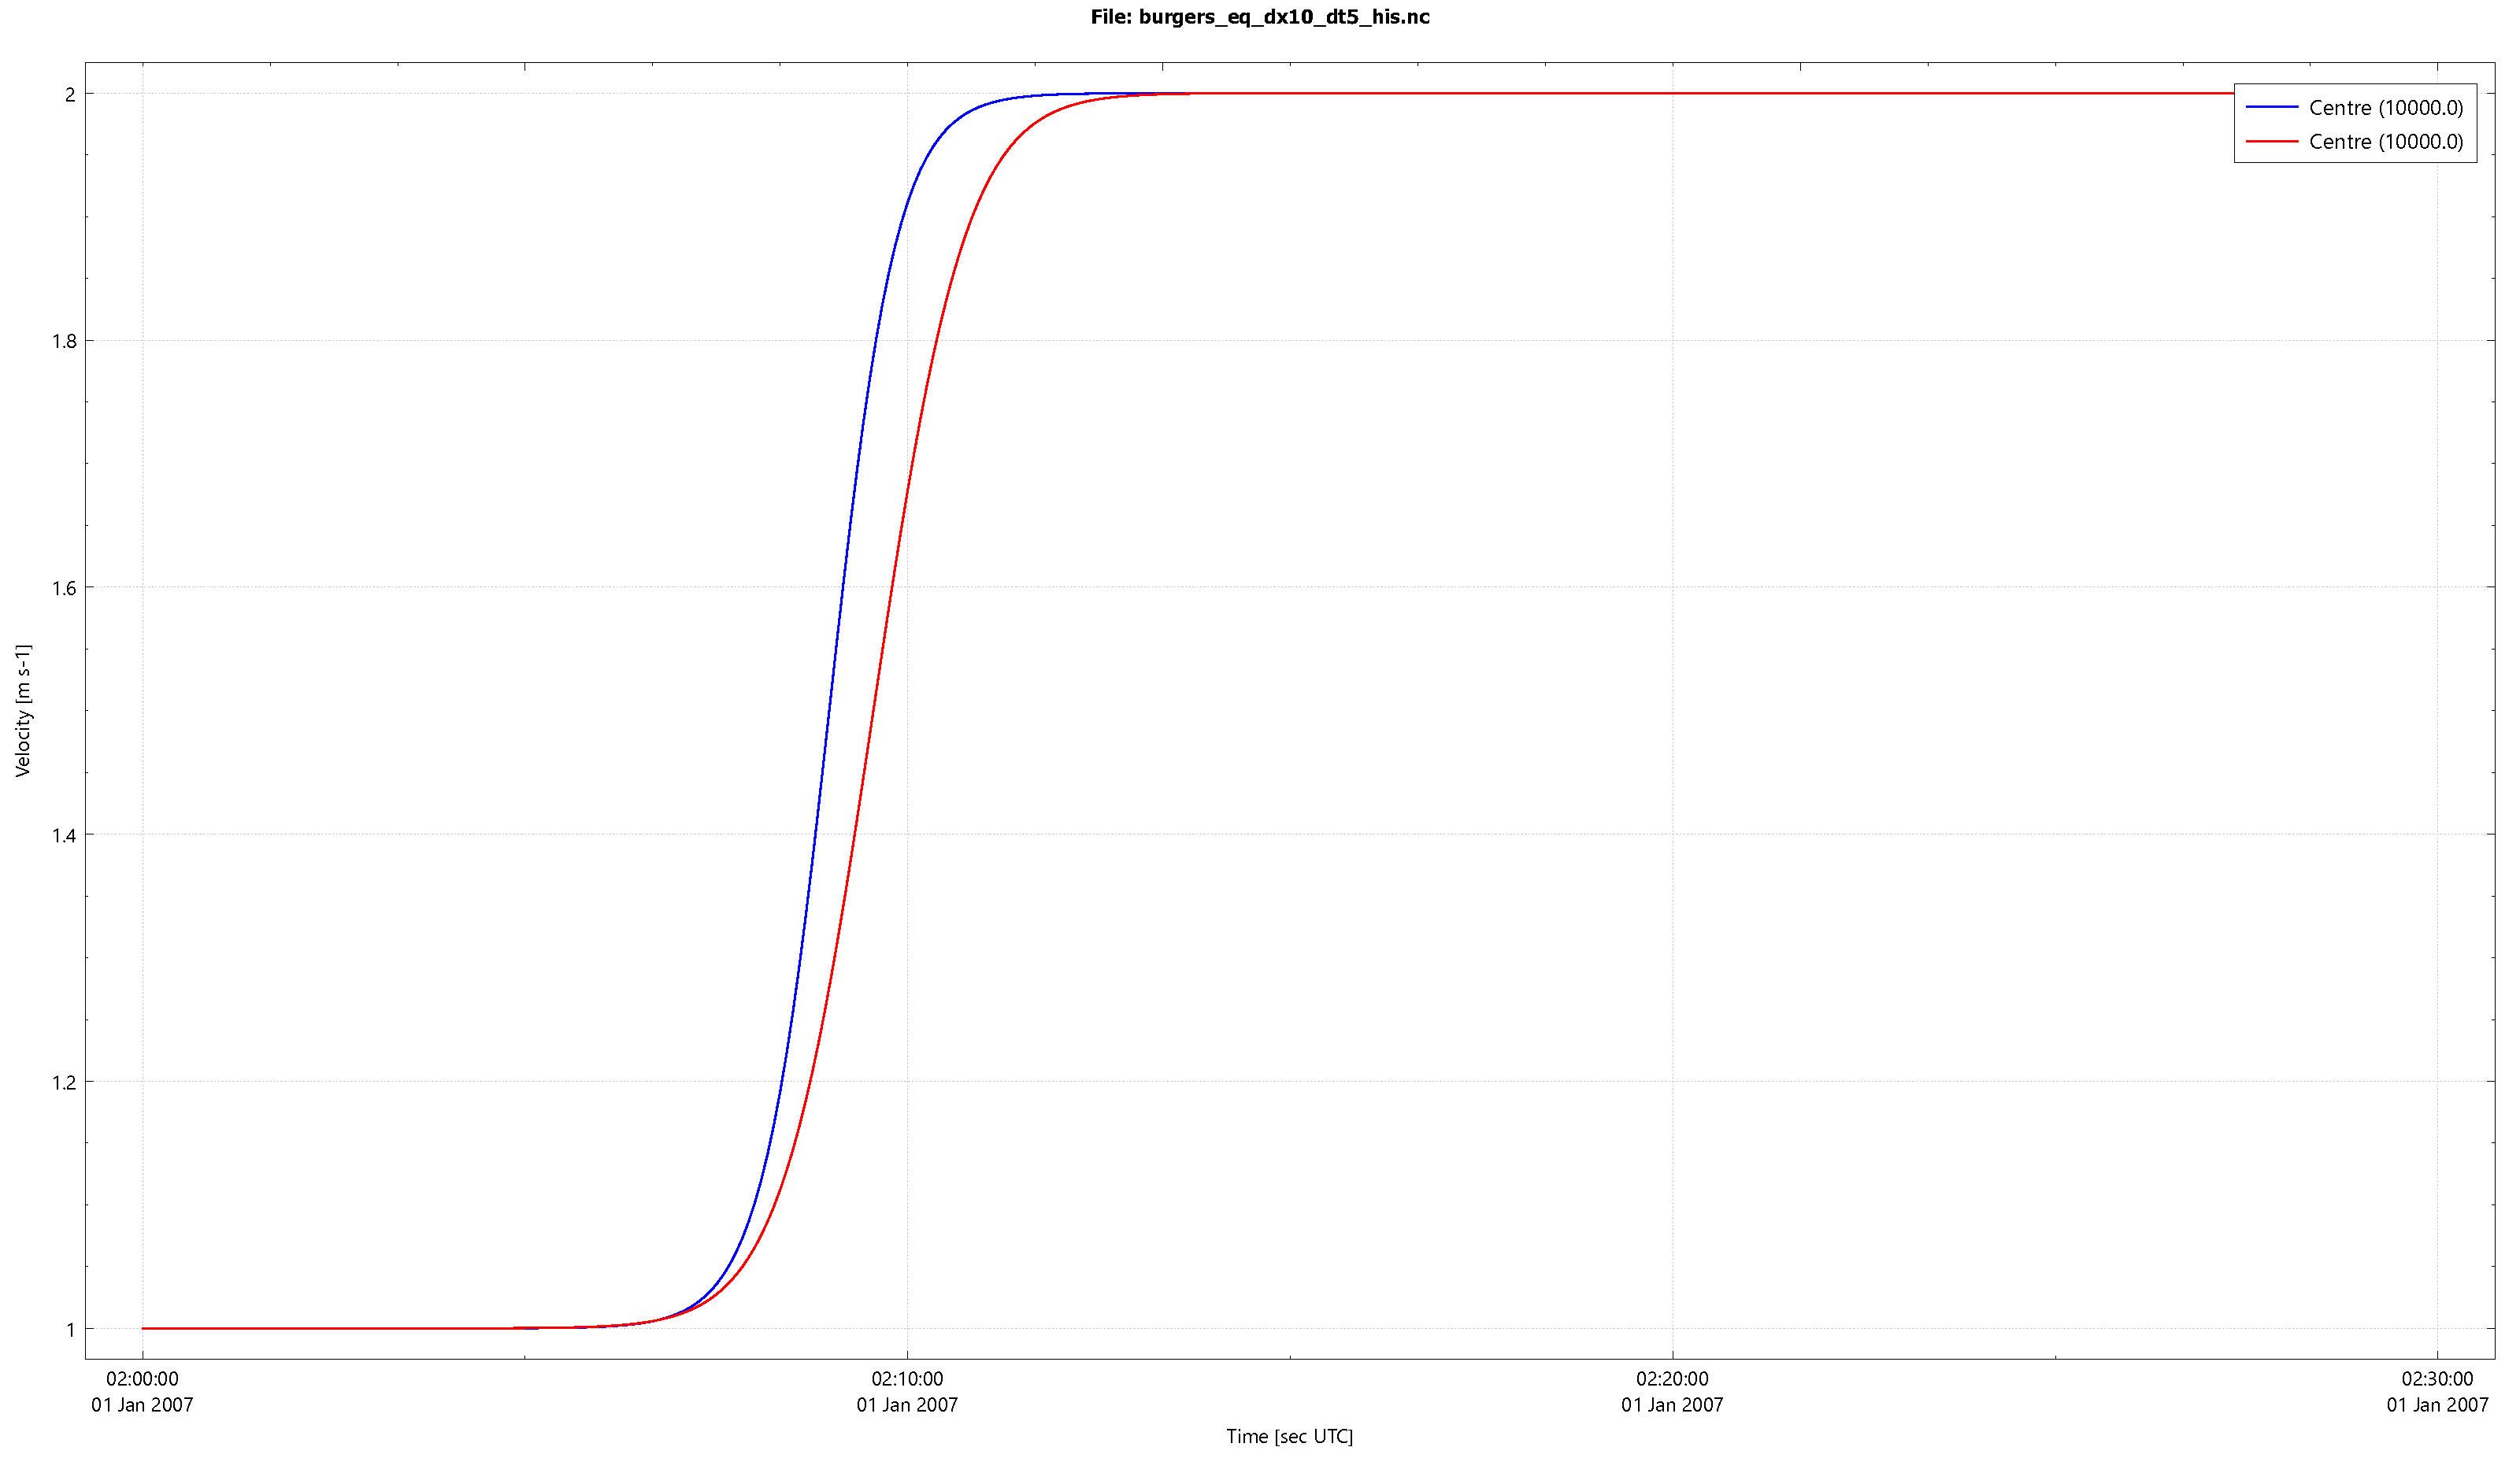
\includegraphics[width=\textwidth]{figures/20260603_115229.pdf}
        \caption{Time histories of the velocity for the observation point  at the centre of the channel. The blue line, without artificial viscosity and the red line with artificial velocity.}
    \end{subfigure}
    \hfill
    \begin{subfigure}{0.49\textwidth}
        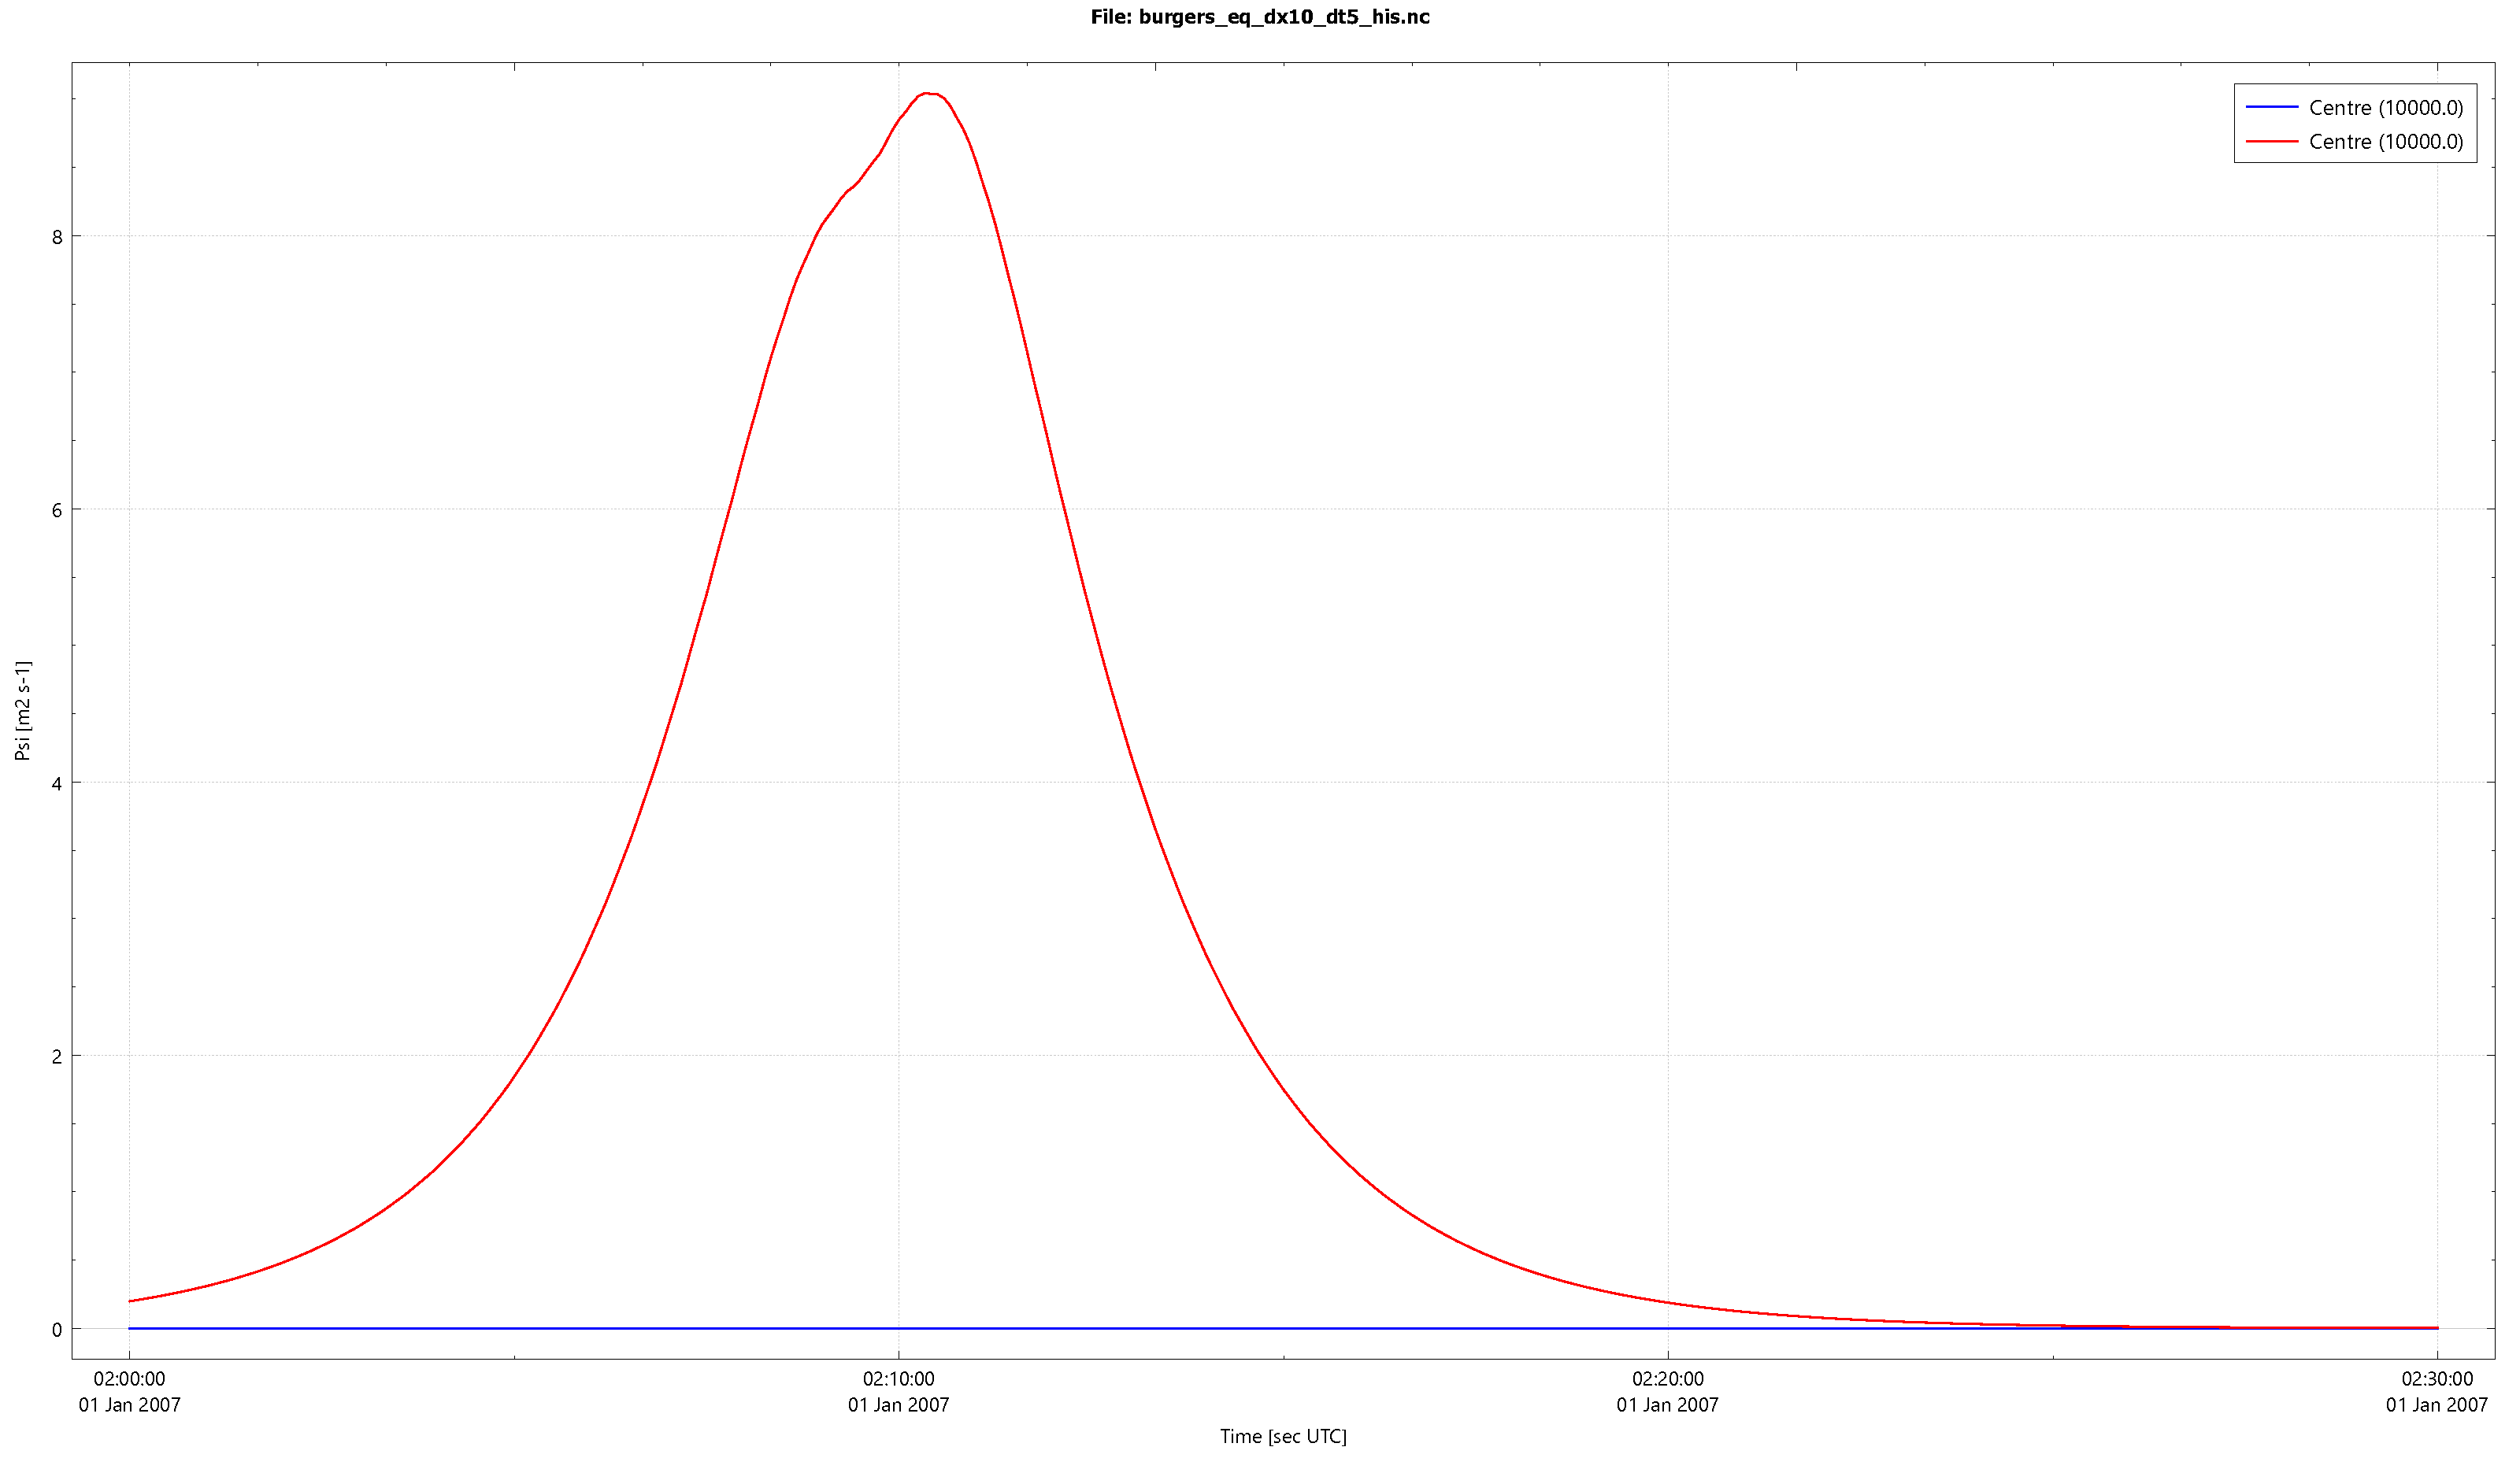
\includegraphics[width=\textwidth]{figures/20260603_115708.pdf}
                \caption{Time histories of the artificial viscosity $\Psi$ for the observation point at the $x=\bqty{10000}{\metre}$ (blue line) and at $x=\bqty{15000}{\metre}$ (red line).
                \newline \phantom{text}}
    \end{subfigure}
    \caption{Time histories for $\nu = \bqty{20}{\square\meter\per\second}$}
\end{figure}
\begin{figure}[H]
    \begin{subfigure}{0.8\textwidth}
        \centering
        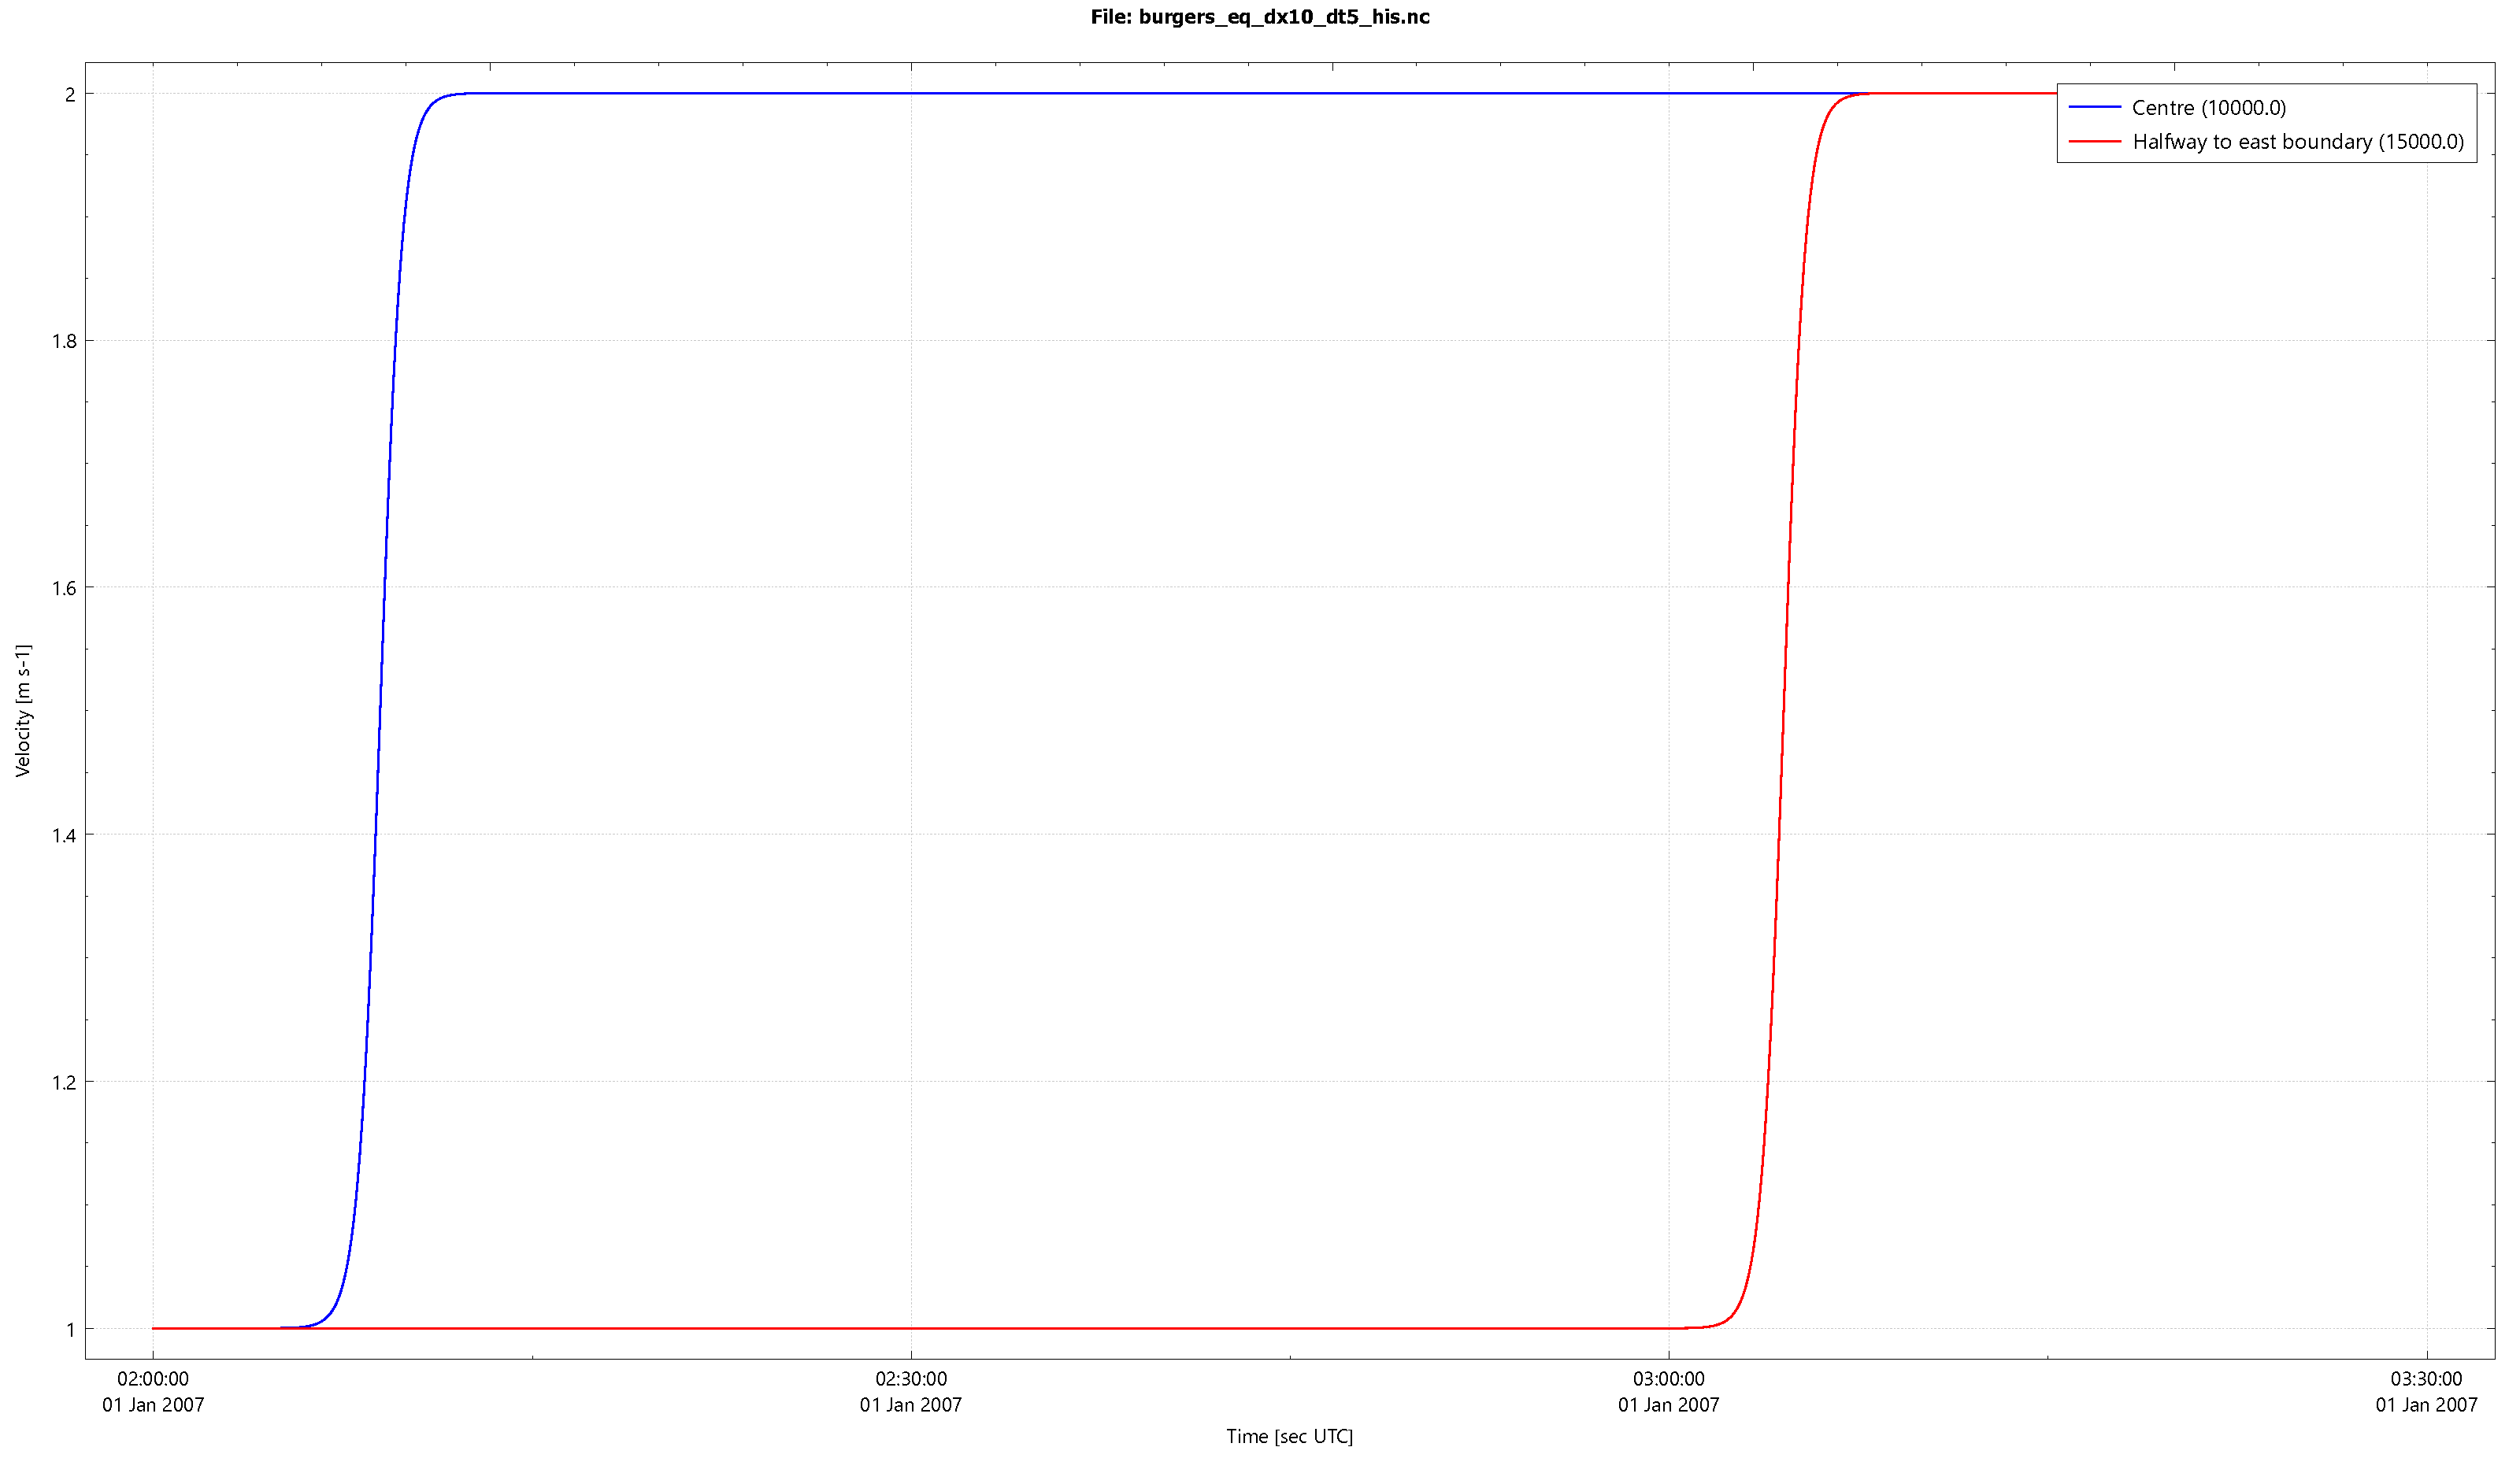
\includegraphics[width=\textwidth]{figures/vel_nu020d0_his_stat_hwaytoeast_centre.pdf}
        \caption{Time histories of the velocity for the observation point at the $x=\bqty{10000}{\metre}$ (blue line) and at $x=\bqty{15000}{\metre}$ (red line). \newline
            \phantom{text}}
    \end{subfigure}
    \begin{subfigure}{0.8\textwidth}
        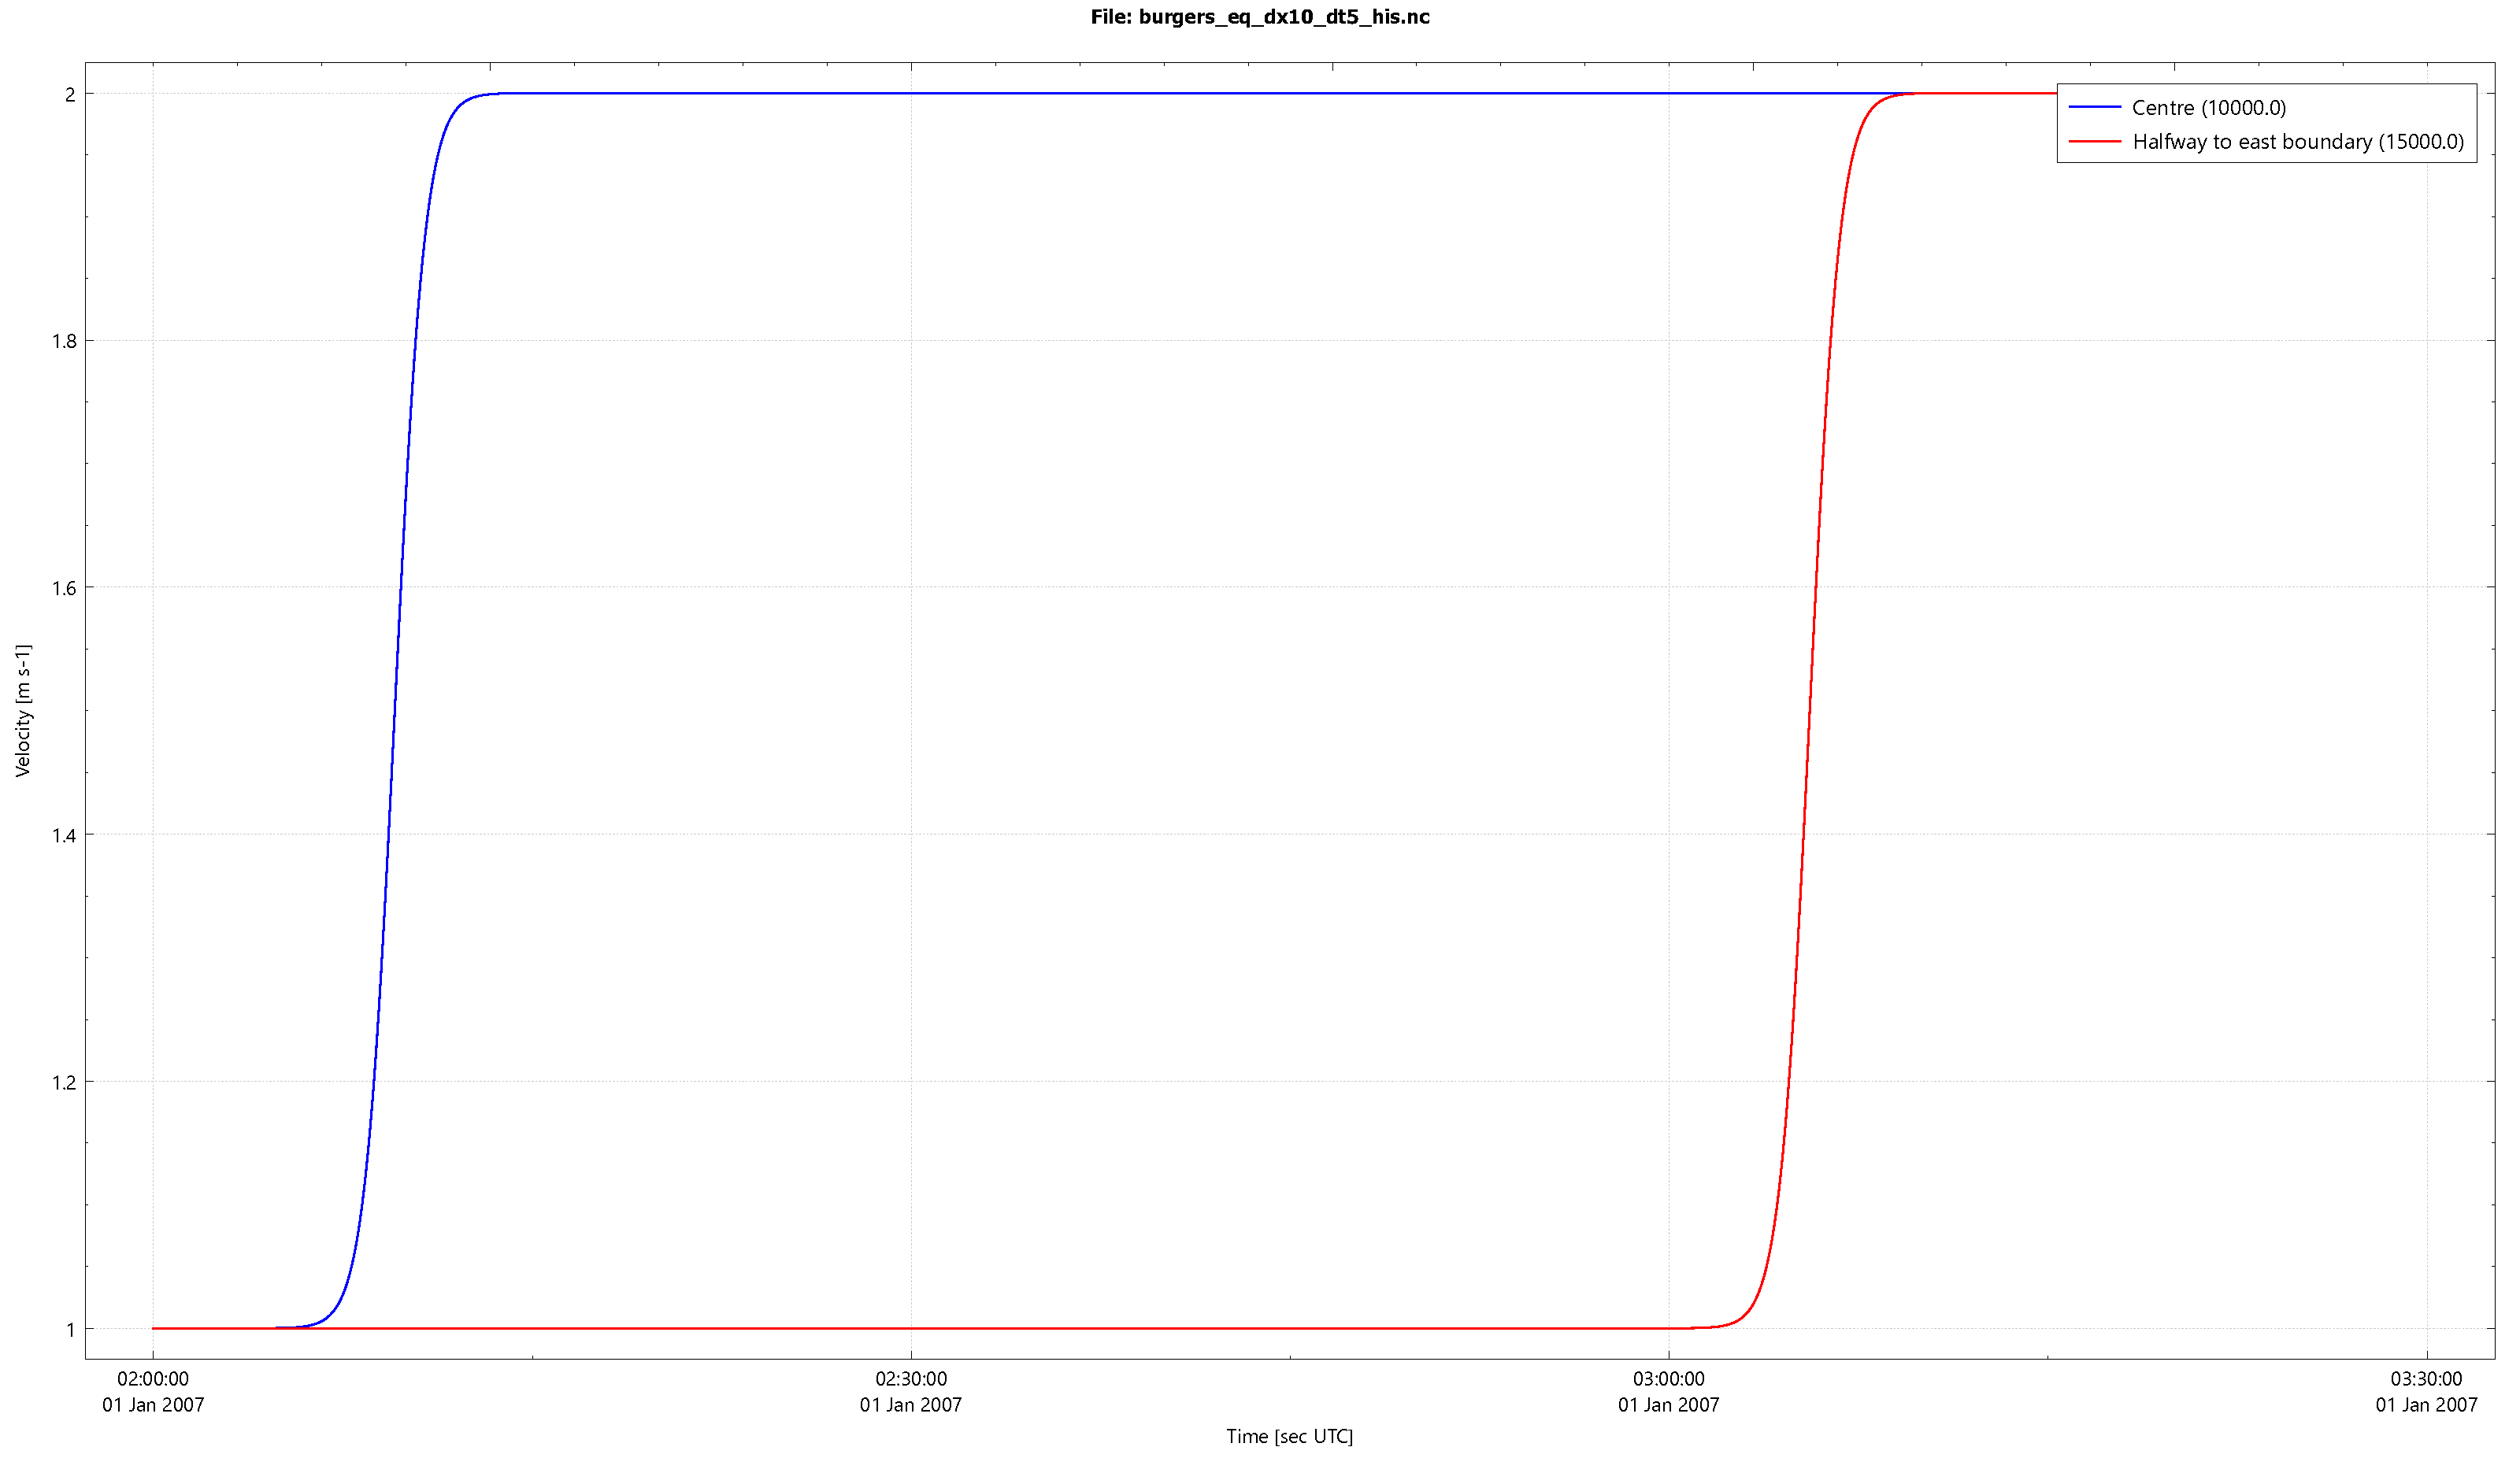
\includegraphics[width=\textwidth]{figures/vel_nu020d0_his_stat_hwaytoeast_centre_psi.pdf}
        \caption{Time histories of the artificial viscosity $\Psi$ for the observation point at the $x=\bqty{10000}{\metre}$ (blue line) and at $x=\bqty{15000}{\metre}$ (red line).}
    \end{subfigure}
    \caption{Time histories for when $\nu = \bqty{20}{\square\meter\per\second}$}
\end{figure}
The wave front has a speed of $u_{\it shock} = \bqty{1.5}{\metre\per\second}$ for both cases, without and with artificial viscosity (i.e. ${1.5000}$ vs $\bqty{1.4999}{\metre\per\second}$).
%----------------------------------------------------------
\section[Experiment with viscosity of 0.1 m2/s]{Experiment with viscosity of \bqty{0.1}{\metre\square\per\second}}
\begin{figure}[H]
    \begin{subfigure}{0.49\textwidth}
        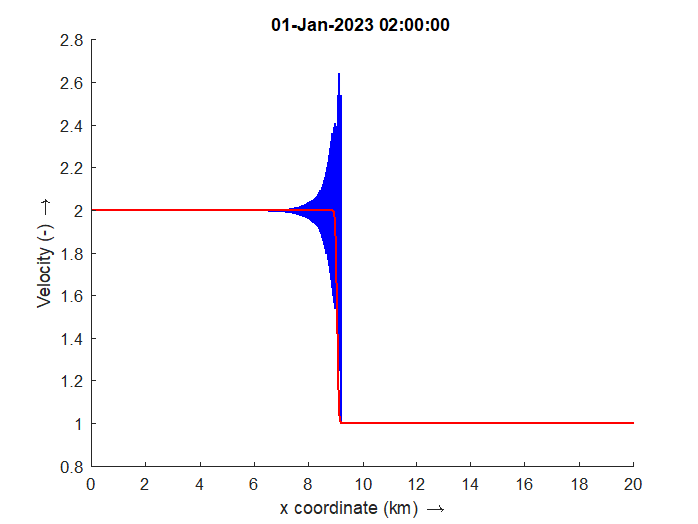
\includegraphics[width=\textwidth]{figures/nu000d1_velocity.png}
        \caption{Velocity along channel at $\bqty{2}{\hour}$. The blue line, without artificial viscosity and the red line with artificial velocity.
        }
    \end{subfigure}
    \hfill
    \begin{subfigure}{0.49\textwidth}
        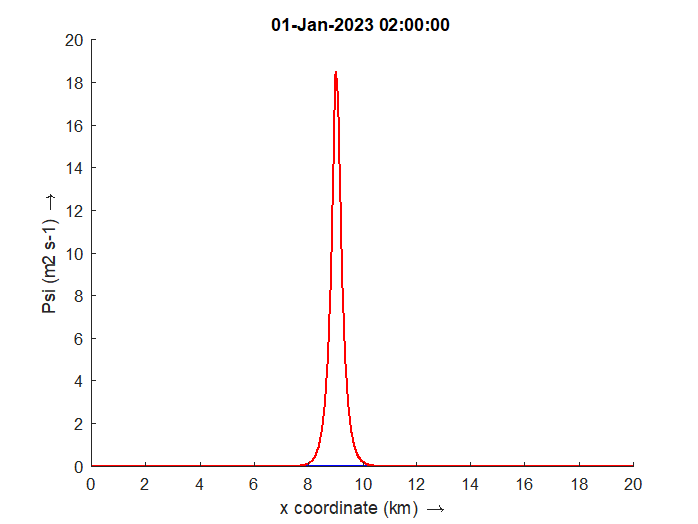
\includegraphics[width=\textwidth]{figures/nu000d1_psi.png}
        \caption{Used artificial viscoity $\Psi$ along channel at $\bqty{2}{\hour}$. The blue line, without artificial viscosity ($\equiv 0$) and the red line with artificial velocity.}
    \end{subfigure}
    \caption{Transect for velocity $\nu = \bqty{0.1}{\square\meter\per\second}$}
\end{figure}

\begin{figure}[H]
    \begin{subfigure}{0.49\textwidth}
        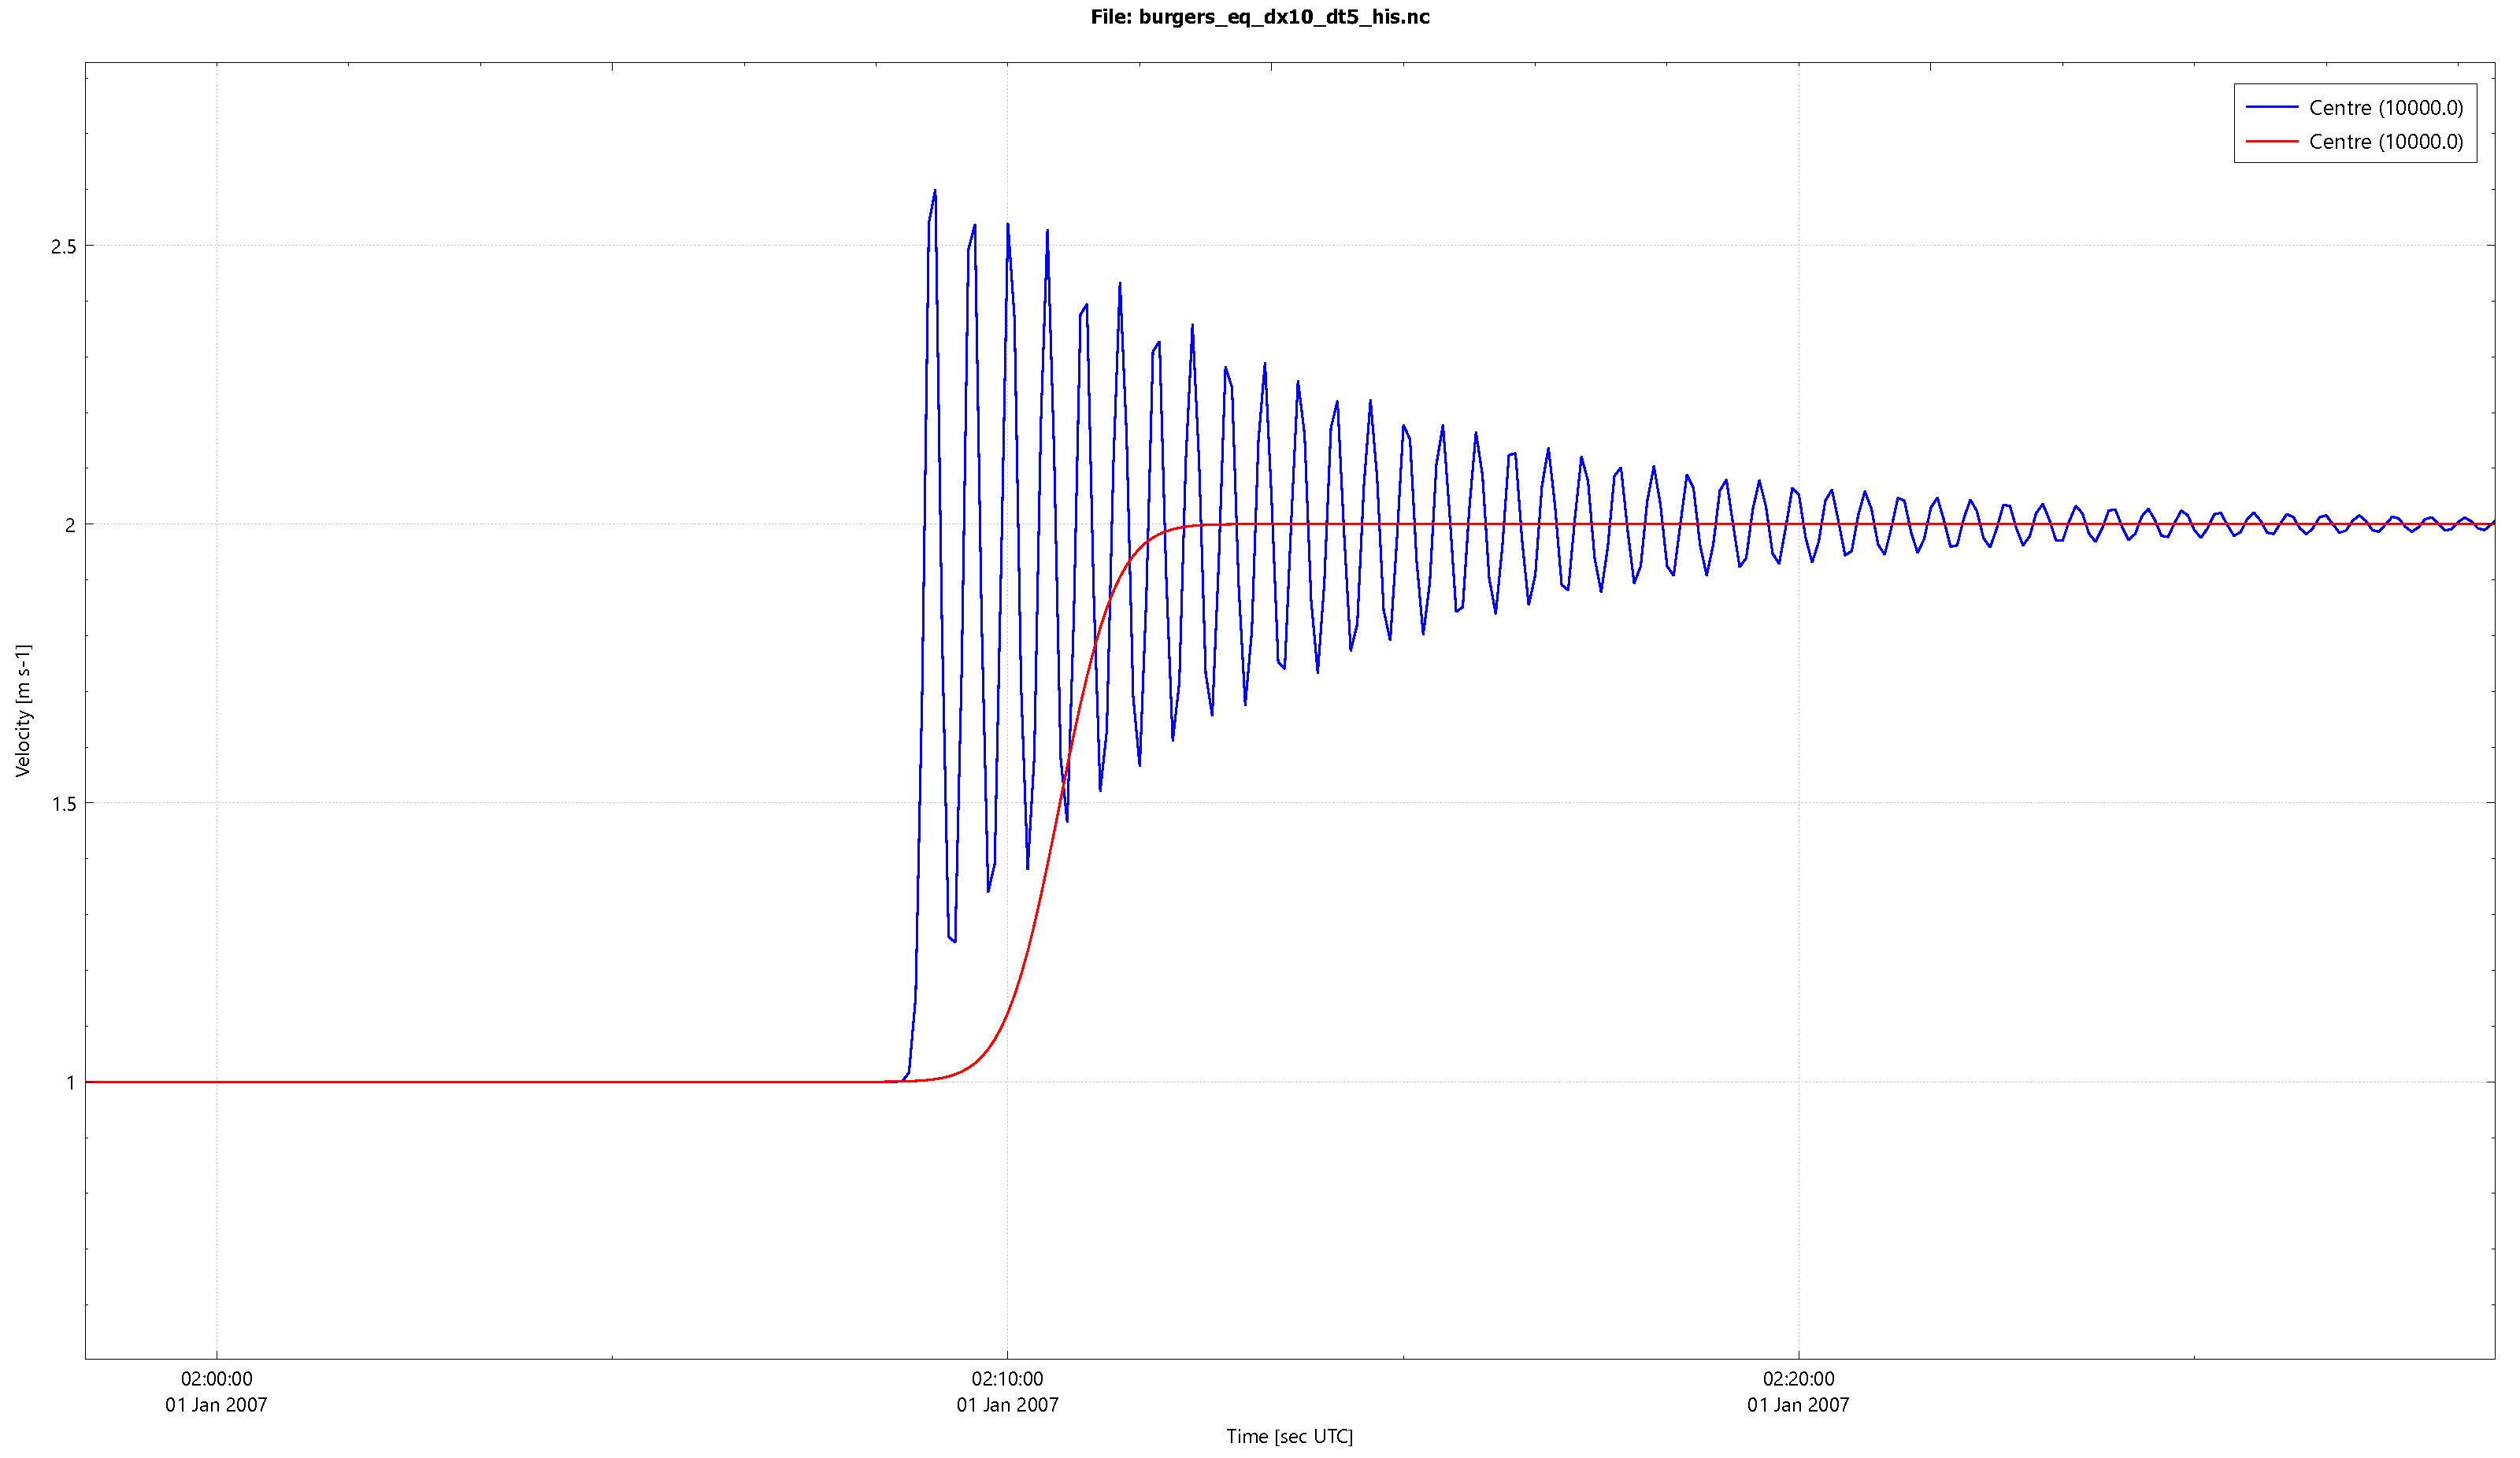
\includegraphics[width=\textwidth]{figures/20260602_224544.pdf}
        \caption{Time histories of the velocity for the observation point  at the centre of the channel. The blue line, without artificial viscosity and the red line with artificial velocity. \newline
        \phantom{text}}
    \end{subfigure}
    \hfill
    \begin{subfigure}{0.49\textwidth}
        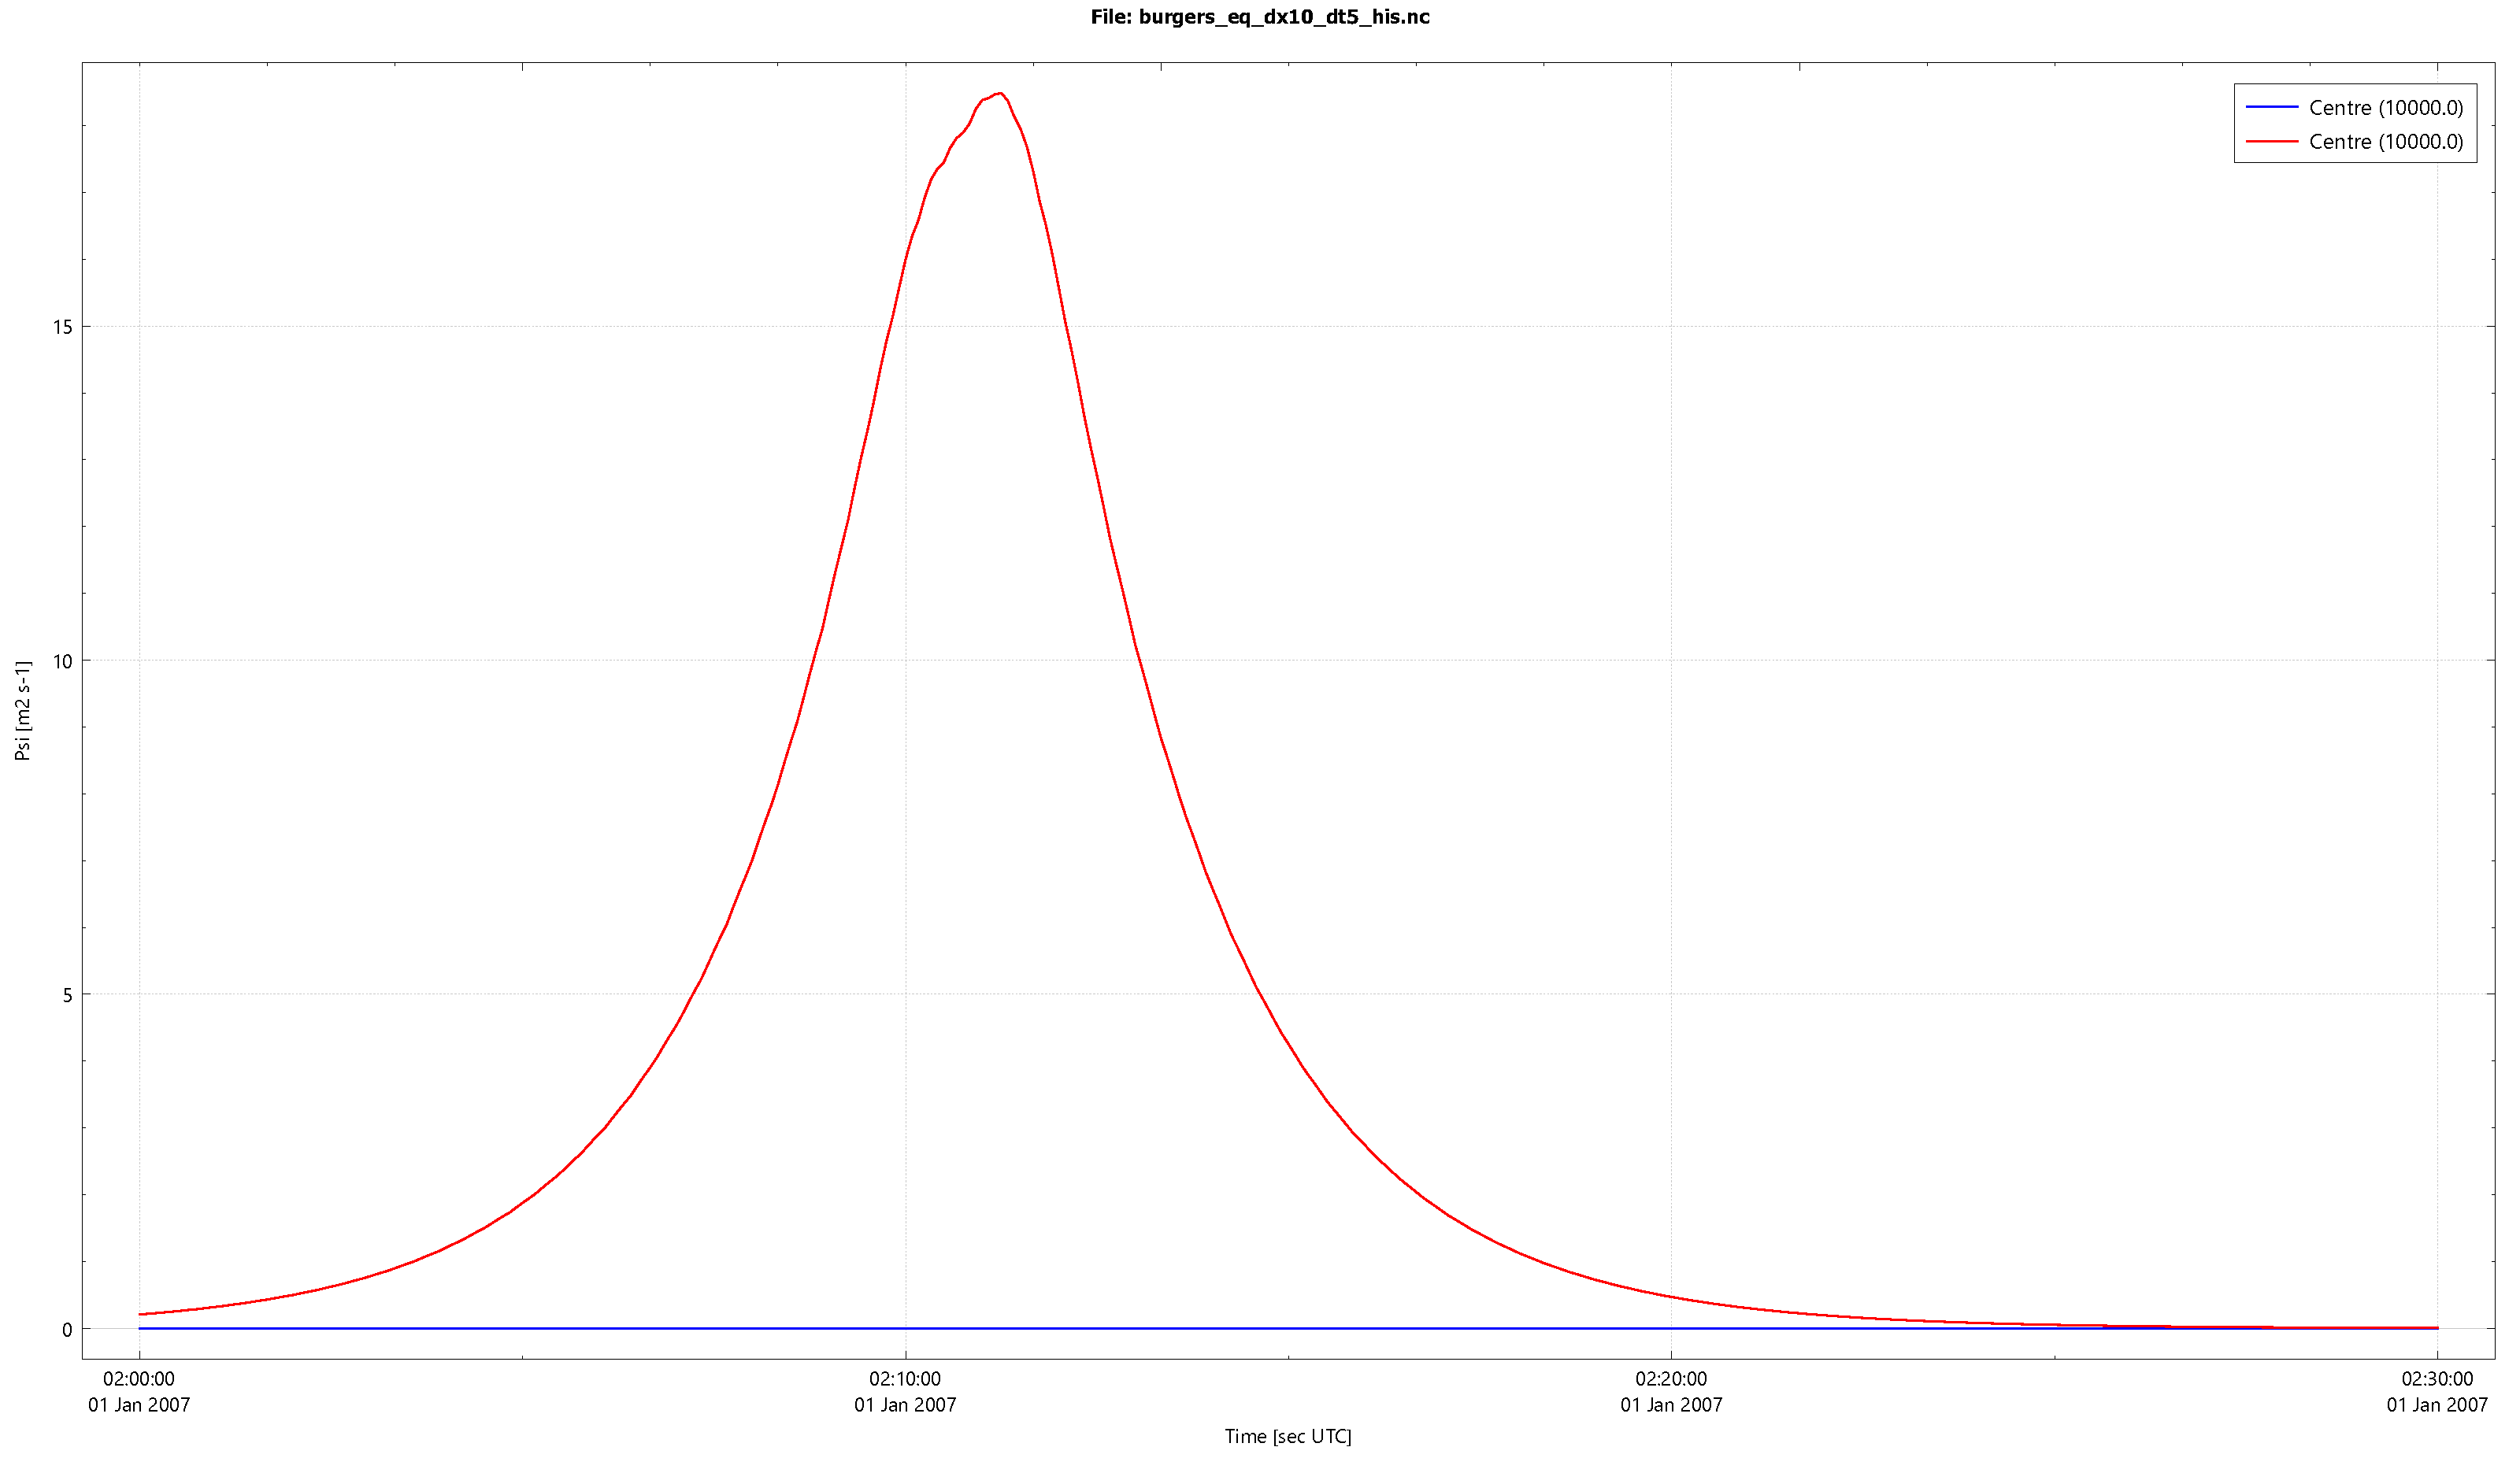
\includegraphics[width=\textwidth]{figures/20260602_225828.pdf}
        \caption{Time histories of the artificial viscosity $\Psi$ for the observation point  at the centre of the channel. The blue line, without artificial viscosity ($\equiv 0$) and the red line with artificial velocity.}
    \end{subfigure}
    \caption{Time histories for $\nu = \bqty{0.1}{\square\meter\per\second}$}
\end{figure}
\begin{figure}[H]
    \begin{subfigure}{0.8\textwidth}
        \centering
        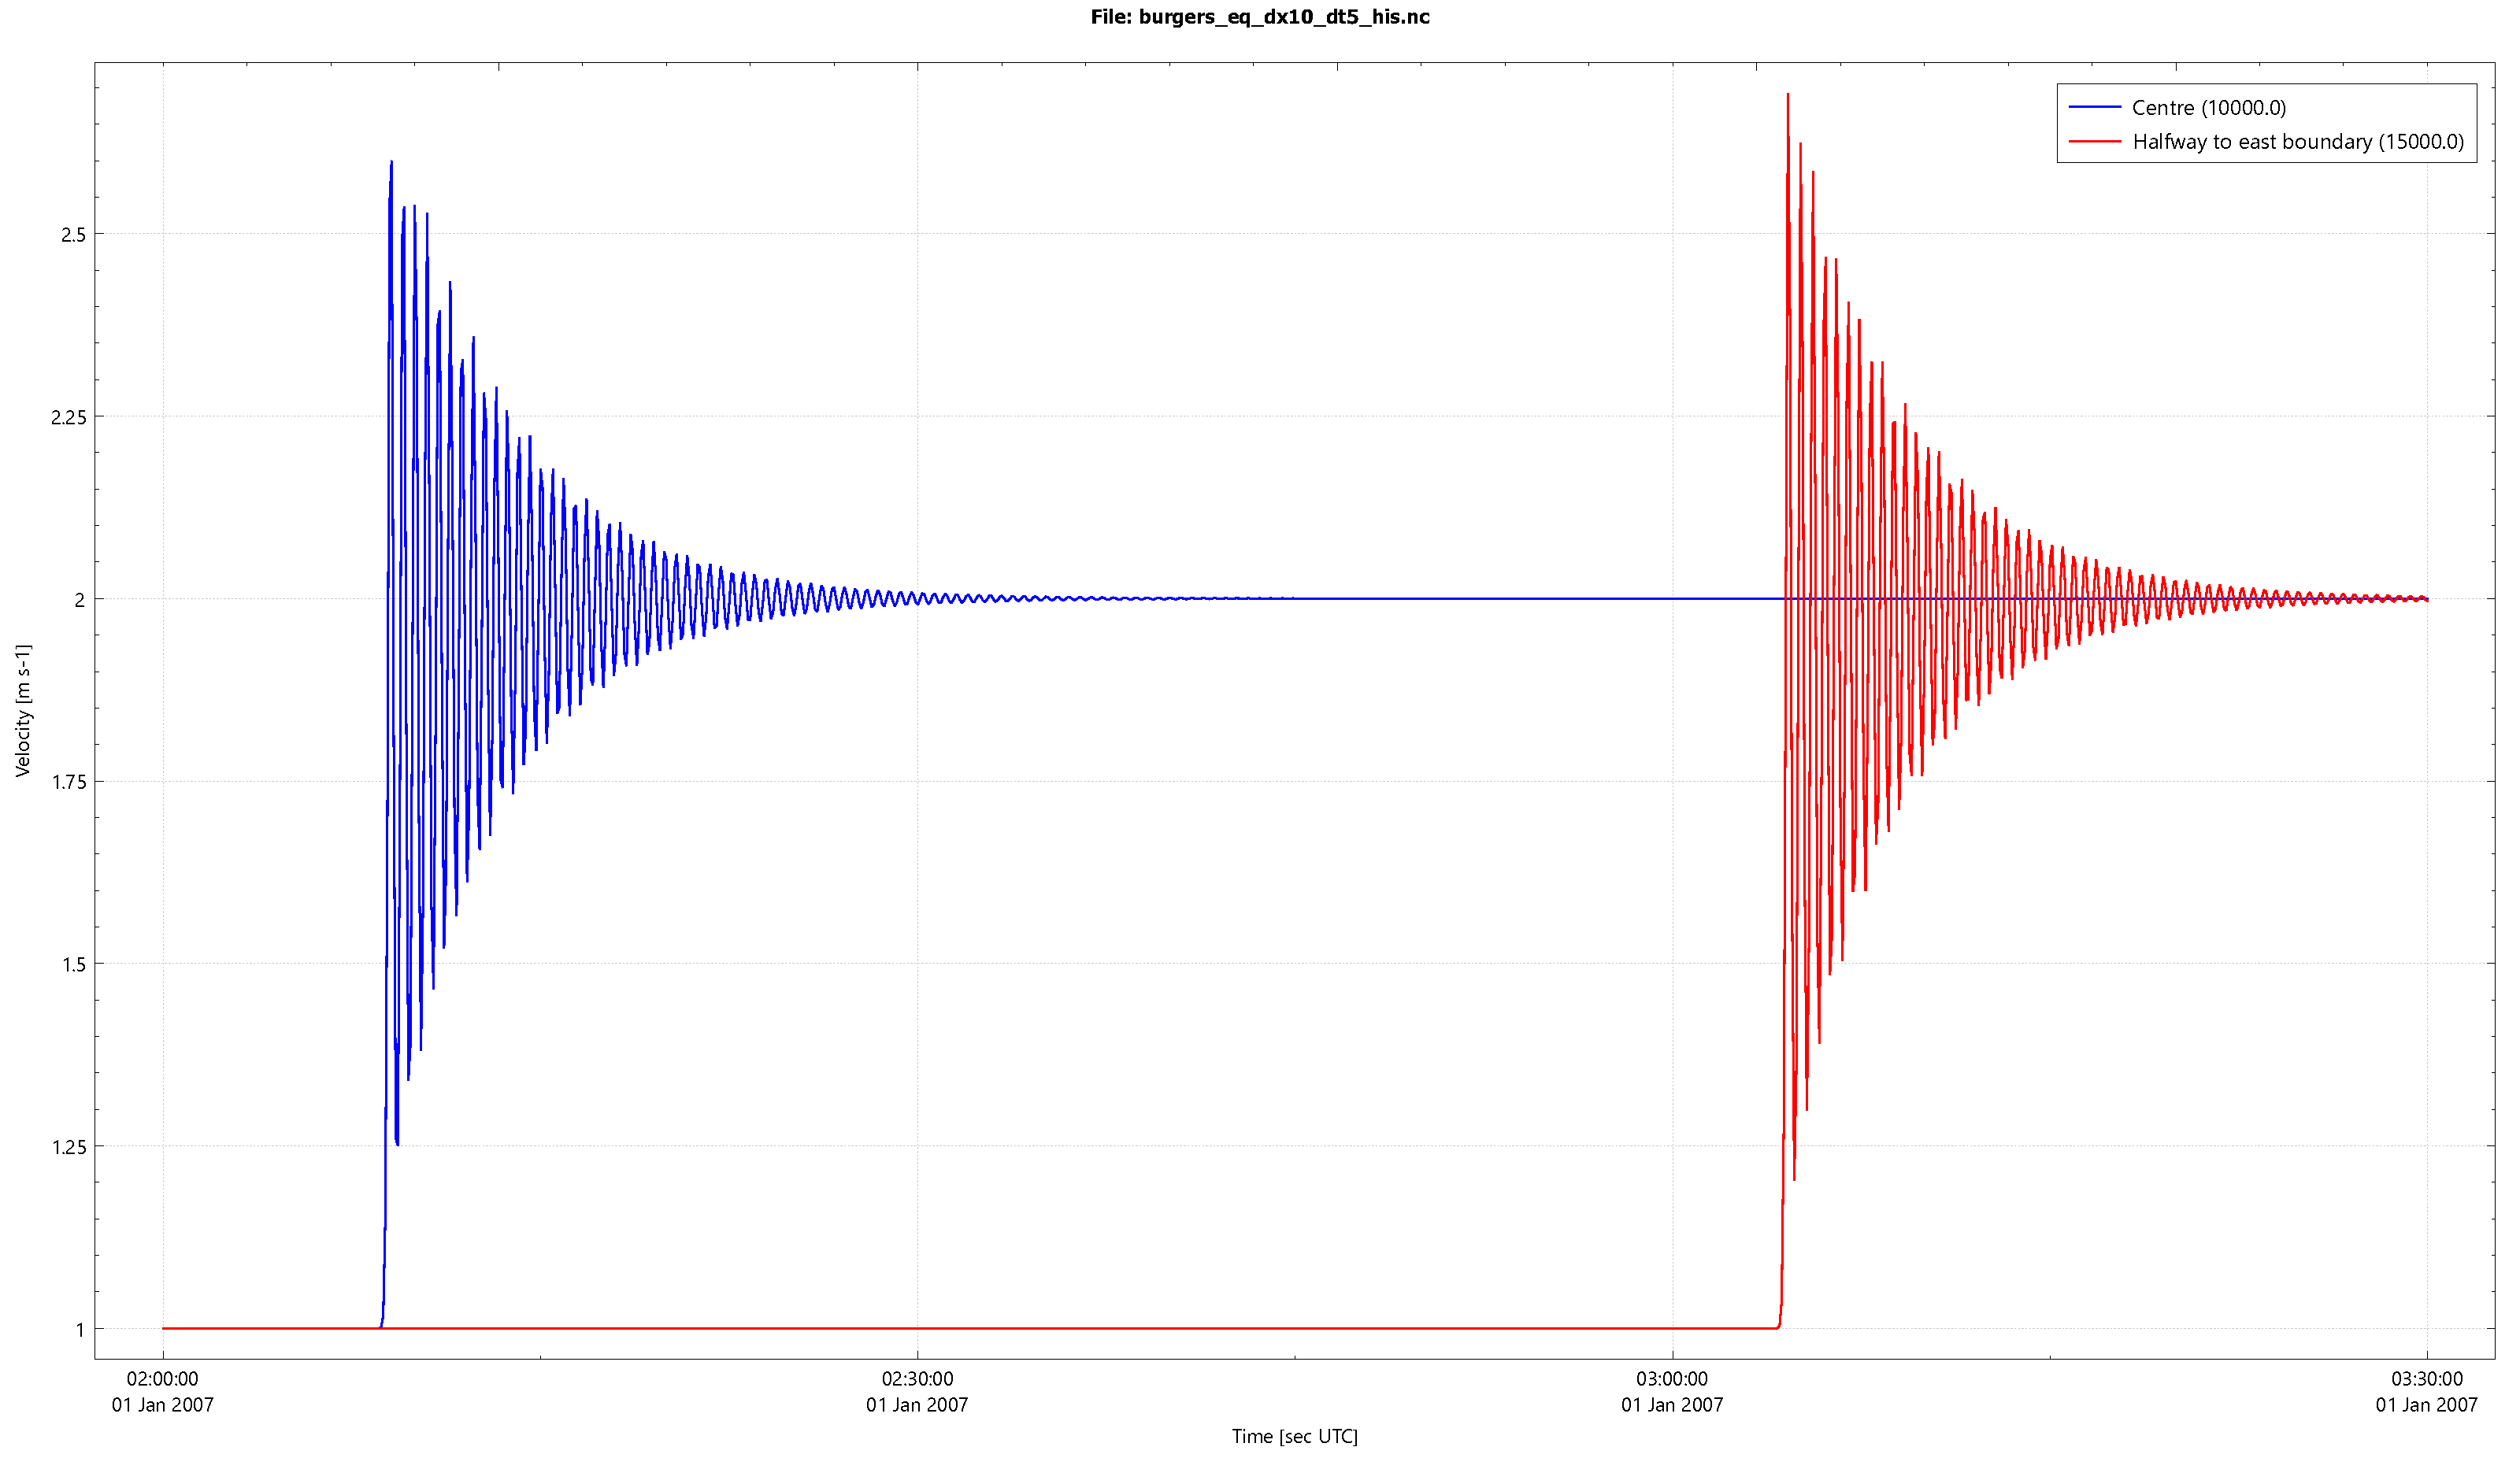
\includegraphics[width=\textwidth]{figures/vel_nu000d1_his_stat_hwaytoeast_centre.pdf}
        \caption{Time histories of the velocity for the observation point at the $x=\bqty{10000}{\metre}$ (blue line) and at $x=\bqty{15000}{\metre}$ (red line). \newline
            \phantom{text}}
    \end{subfigure}
    \begin{subfigure}{0.8\textwidth}
        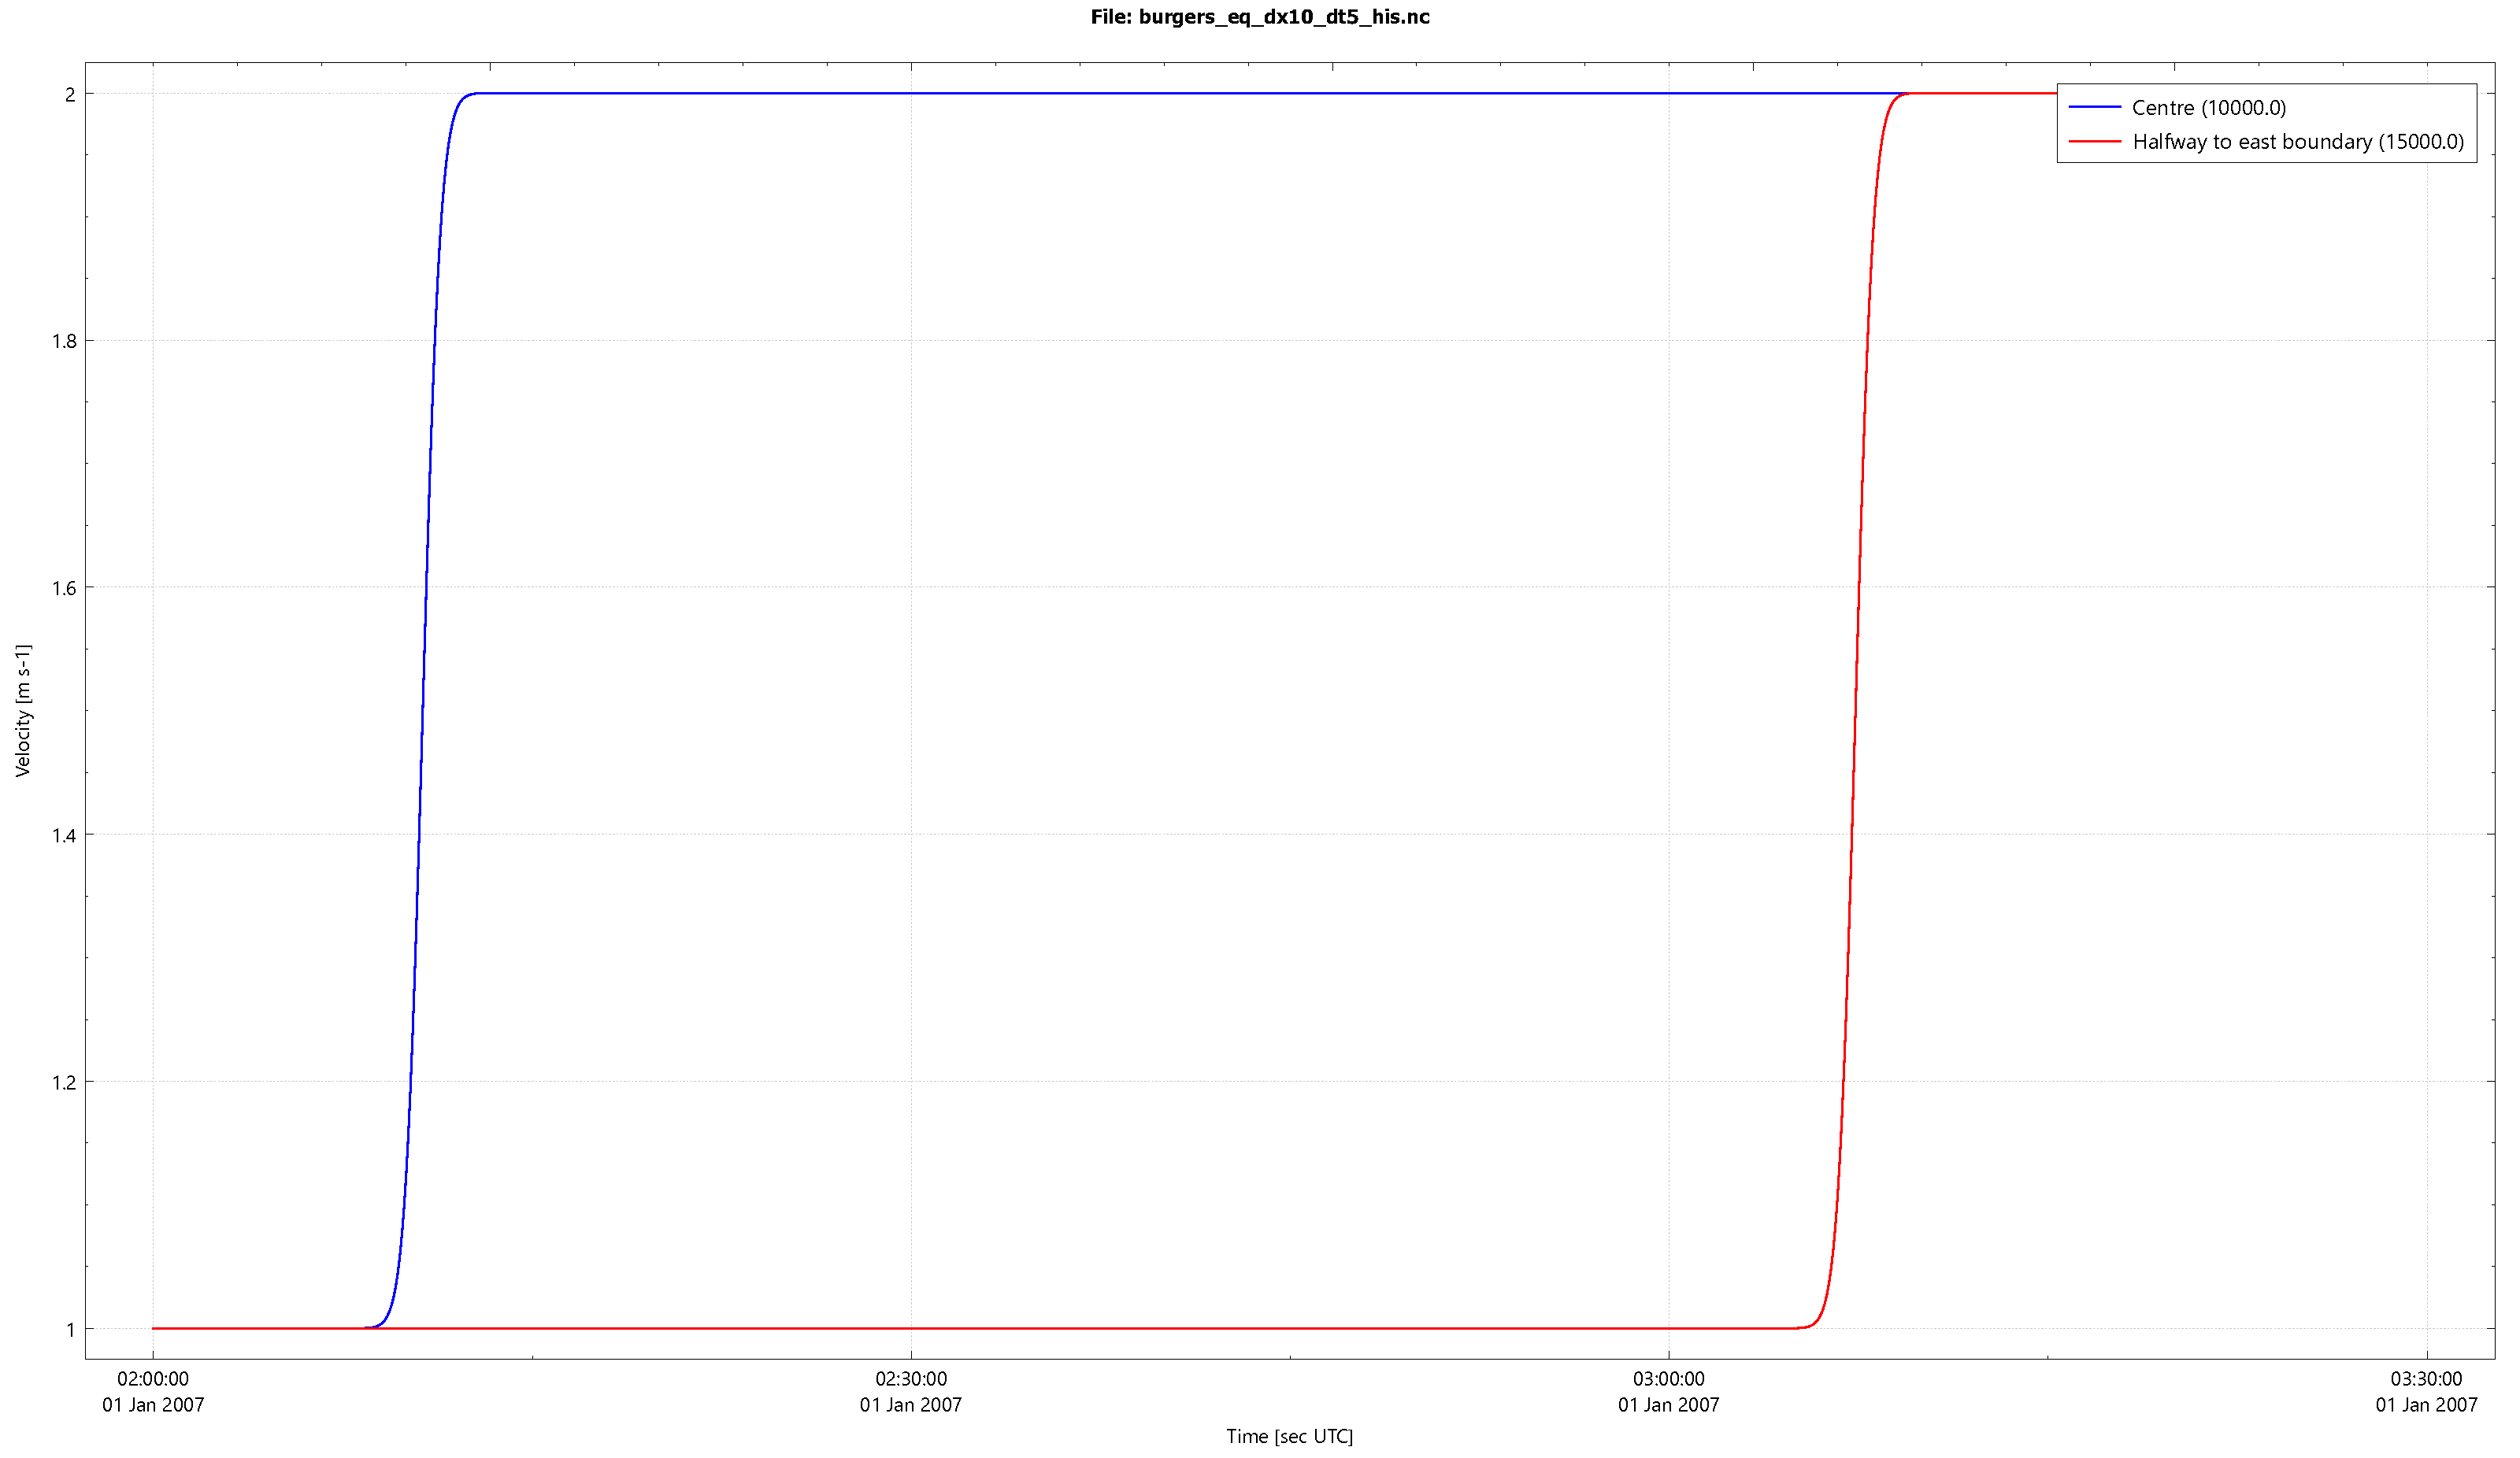
\includegraphics[width=\textwidth]{figures/vel_nu000d1_his_stat_hwaytoeast_centre_psi.pdf}
                \caption{Time histories of the artificial viscosity $\Psi$ for the observation point at the $x=\bqty{10000}{\metre}$ (blue line) and at $x=\bqty{15000}{\metre}$ (red line).}
    \end{subfigure}
    \caption{Time histories for when $\nu = \bqty{0.1}{\square\meter\per\second}$}
\end{figure}
The wave front has a speed of $u_{\it shock} = \bqty{1.5}{\metre\per\second}$ for both cases, without and with artificial viscosity (i.e. ${1.5000}$ vs $\bqty{1.5000}{\metre\per\second}$).

%-------------------------------------------------------------------------------
%\subsection{Constant viscosity $\nu$}
%-------------------------------------------------------------------------------
\section{Experiment with non linear source term}
This experiment is taken from \citet{Colombo2026} and read
\begin{align}
    \pdiff{u}{t} + u \pdiff{u}{x} - \nu \pdiff[2]{u}{x}= u^2, \quad u >0
\end{align}
With viscosity coefficient $\nu = \bqty{0.0}{\square\metre\per\second}$ and initial condition
\begin{align}
u(x,0) = \exp(x) + 0.3 \exp( -200 (x + 0.5)^2), \quad x\in = [-1,1]
\end{align}
and boundary condition at the left side
\begin{align}
    u(-1,t) = \exp(-1).
\end{align}


\notyet